\chapter{Metodologia}\label{chp:desenvolvimento}

Este capítulo descreve a metodologia implementada no repositório que acompanha a
dissertação. A organização segue o fluxo executável do projeto, mas a exposição
é apresentada em forma científica: primeiro são descritos os contratos de dados,
depois as decisões de pré-processamento, particionamento, treinamento e
inferência. Sempre que uma escolha é específica da implementação, ela é tratada
como decisão do repositório, não como reprodução exata de um método publicado.

\section{Visão geral do fluxo de trabalho}\label{sec:met_visao_geral}

O fluxo de trabalho foi construído como uma sequência de fases com entradas e
saídas explícitas. Scripts numerados na raiz do repositório orquestram cada
etapa, enquanto a lógica reutilizável fica concentrada em módulos sob
\texttt{helpers/}. Essa separação reduz a dependência de execução manual e
facilita auditar o caminho que liga uma WSI original à máscara prevista pelo
\textit{ensemble} final.

A \Figura{fig:fluxo-atual} resume o desenho metodológico. O processo começa com
lâminas e anotações, passa por controle de qualidade e extração de
\textit{patches}, consolida manifestos e HDF5, produz divisões por paciente,
treina modelos supervisionados, otimiza um \textit{ensemble} em validação e,
por fim, avalia uma receita congelada no teste. A tabela de fases detalha a
mesma sequência em termos operacionais.

\begin{figure}[!htb]
    \centering
    \small
    \setlength{\tabcolsep}{3pt}
    \begin{tabular}{ccccc}
    \fbox{\begin{minipage}{0.16\textwidth}\centering WSIs\\anotações\end{minipage}} &
    $\rightarrow$ &
    \fbox{\begin{minipage}{0.18\textwidth}\centering QC\\artefatos\end{minipage}} &
    $\rightarrow$ &
    \fbox{\begin{minipage}{0.20\textwidth}\centering patches\\máscaras\\HDF5\end{minipage}} \\
    &&&&\\[-0.3em]
    \multicolumn{5}{c}{$\downarrow$}\\[-0.2em]
    \fbox{\begin{minipage}{0.16\textwidth}\centering limpeza\\por grafos\end{minipage}} &
    $\rightarrow$ &
    \fbox{\begin{minipage}{0.18\textwidth}\centering splits\\paciente\\normalização\end{minipage}} &
    $\rightarrow$ &
    \fbox{\begin{minipage}{0.20\textwidth}\centering treino\\ensemble\\inferência\end{minipage}}
    \end{tabular}
    \caption[Fluxo metodológico atual]{Visão macro do fluxo metodológico atual. A figura é uma síntese visual; os contratos detalhados são descritos nas seções seguintes e implementados nos scripts de Fase 1 a Fase 10.}
    \label{fig:fluxo-atual}
\end{figure}

\begin{table}[!htb]
\centering
\caption{Resumo dos estágios metodológicos implementados.}
\label{tab:estagios_pipeline}
\begin{tabular}{p{1.6cm}p{5.0cm}p{6.8cm}}
\toprule
Fase & Finalidade & Saída principal \\
\midrule
1 & Detecção de artefatos em WSI & GeoJSONs de artefatos e estado em SQLite \\
2 & Ingestão e extração de \textit{patches} & HDF5 por lâmina, máscaras e manifesto mestre \\
3.1--3.3 & Amostragem para revisão e limpeza por grafos & Pastas de revisão, parâmetros e decisões aceitas/rejeitadas \\
4 & Particionamento e artefatos de normalização & Divisão por paciente e estados de normalização em tempo de execução \\
5 & Verificação científica de sanidade & Relatório fail-closed sobre contratos e dados \\
6 & Amostragem inteligente do treino & Estado de seleção e armazenamento compacto opcional \\
7 & Busca de taxa de aprendizado e pesos de perda & Relatórios de triagem e histórico de perda \\
8 & Treinamento supervisionado & Checkpoints e metadados de modelos individuais \\
9 & Otimização de \textit{ensemble} em validação & Receita congelada de \textit{ensemble} \\
10 & Inferência final em teste & Métricas, figuras e relatórios finais \\
\bottomrule
\end{tabular}
\end{table}

\section{Aquisição, ingestão e controle de qualidade}\label{sec:met_ingestao_qc}

A primeira etapa metodológica trata a WSI como um objeto de dados volumoso,
heterogêneo e sujeito a falhas de leitura. A Fase 1 processa lâminas arquivadas
sem exigir que todo o conjunto seja extraído permanentemente para disco. Cada
lâmina suportada é extraída temporariamente, submetida à inferência de
artefatos, convertida em polígonos GeoJSON e removida ao final do
processamento. O estado da execução é registrado em SQLite, permitindo retomar
processamentos interrompidos sem duplicar artefatos.

A detecção de artefatos combina uma etapa de localização de tecido com uma etapa
de classificação de qualidade. A motivação científica vem de trabalhos de QC em
WSI, como GrandQC \cite{weng2024grandqc}; a implementação aqui, porém, é usada
como componente operacional para registrar cobertura de artefatos. Essas
coberturas não são tratadas automaticamente como exclusão definitiva de dados em
todas as fases. Elas entram como metadados de proveniência que podem ser usados
em experimentos posteriores, por exemplo em perda sensível a artefatos.

A Fase 2 realiza a ingestão supervisionada. Ela localiza pares de lâmina e
anotação, registra assinaturas de entrada, cria linhas pendentes no banco de
progresso e valida se saídas pré-existentes ainda são compatíveis com a fonte
atual. Em seguida, o motor de extração percorre uma grade de janelas definida por
tamanho e passo. Antes de ler pixels da WSI, a janela é comparada com as
geometrias anotadas, reduzindo I/O desnecessário em regiões sem relação com a
tarefa.

Um \textit{patch} só é aceito quando satisfaz três condições. Primeiro, a janela
precisa ter associação semântica não ambígua a uma classe. Segundo, deve conter
conteúdo tecidual suficiente, estimado por limiarização e operações
morfológicas, como discutido na \Secao{sec:preprocessamento_patologia}.
Terceiro, sua identidade precisa seguir um contrato determinístico de nome e
proveniência. A \Figura{fig:patch-mask} ilustra o produto elementar dessa etapa:
um recorte RGB e sua máscara binária correspondente.

\begin{figure}[!htb]
    \centering
    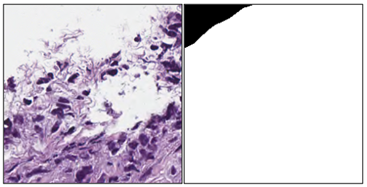
\includegraphics[width=0.55\textwidth]{figuras/image_plus_mask.png}
    \caption[Exemplo de \textit{patch} e máscara]{Exemplo qualitativo de pareamento entre \textit{patch} histológico e máscara binária de supervisão. A figura é ilustrativa e não representa resultado quantitativo final.}
    \label{fig:patch-mask}
\end{figure}

As máscaras de câncer são persistidas como máscaras binárias. Amostras não
cancerosas recebem máscaras zeradas, preservando a mesma estrutura de dados. Os
arquivos HDF5 mantêm alinhamento por linha entre \texttt{images},
\texttt{masks}, \texttt{labels}, \texttt{patient\_ids} e \texttt{filenames}. A
estabilidade desses nomes é um contrato científico: se imagem, máscara e
identificador se desalinharem, as fases de limpeza, treino e avaliação perdem
validade.

\section{Tratamento de ambiguidade e limpeza por grafos}\label{sec:met_limpeza_grafos}

A qualidade da anotação é tão importante quanto a qualidade visual da lâmina.
Quando regiões positivas e negativas se sobrepõem com área positiva, a
supervisão resultante é contraditória. O fluxo atual remove os polígonos
conflitantes no momento de finalização das anotações, preservando regiões
independentes da mesma lâmina. Essa regra é uma política local de integridade:
a literatura sobre rótulos ruidosos em segmentação médica motiva a preocupação
geral, mas não define esse critério específico \cite{yu2020noisy}.

Depois da extração inicial, as Fases 3.1 a 3.3 tratam contaminação por fundo em
amostras cancerosas. A Fase 3.1 seleciona uma amostra para revisão humana,
preservando pareamento entre imagem, máscara e proveniência. A Fase 3.2 ajusta
parâmetros de uma regra automática com base nas decisões revisadas. A Fase 3.3
aplica essa regra ao conjunto canceroso completo sem reescrever os HDF5
originais.

O escore de contaminação mede a fração da região de interesse que cai em
segmentos classificados como fundo:
\begin{equation}
    c = \frac{\sum_x B(x)R(x)}{\sum_x R(x)} ,
    \label{eq:contaminacao}
\end{equation}
em que $R(x)$ indica a região de interesse após erosão e $B(x)$ indica se o
segmento que contém o pixel $x$ foi classificado como fundo. Os segmentos são
obtidos por uma formulação inspirada em Felzenszwalb
\cite{felzenszwalb2004efficient}. O escore $c$ é uma heurística operacional, não
uma medida clínica.

Os parâmetros de segmentação e o limiar de rejeição são escolhidos por
otimização Bayesiana com validação agrupada
\cite{snoek2012practical,roberts2017crossvalidation}. A regra final rejeita uma
amostra quando:
\begin{equation}
    \hat{y}=\mathrm{Rejeitada}\quad \text{se, e somente se,}\quad c>\tau .
    \label{eq:regra_rejeicao}
\end{equation}
Valores exatamente iguais a $\tau$ permanecem aceitos pelo contrato atual. Essa
decisão deve ser mantida explícita porque pequenas diferenças em desigualdades
podem alterar linhas na fronteira do critério.

\section{Empacotamento, particionamento e normalização}\label{sec:met_particionamento_normalizacao}

Após extração e limpeza, o empacotamento consolida linhas aceitas em uma fonte
canônica para as fases seguintes. O HDF5 é usado por permitir acesso por linha,
armazenamento de matrizes grandes e metadados estruturados \cite{folk2011hdf5}.
Essa etapa não redimensiona imagens nem altera máscaras; ela preserva os arrays
produzidos pela extração e copia metadados necessários para rastreabilidade.

A Fase 4 cria uma única divisão \texttt{TRAIN}, \texttt{VALIDATION} e
\texttt{TEST}. A unidade de isolamento é o identificador de paciente persistido
durante a ingestão. Todas as linhas do mesmo identificador permanecem no mesmo
conjunto, reduzindo risco de vazamento por correlação entre \textit{patches}
\cite{roberts2017crossvalidation,dawood2026confounding}. A busca da divisão usa
Optuna/TPE para explorar combinações e minimizar desequilíbrios relevantes entre
conjuntos \cite{akiba2019optuna,bergstra2011algorithms}.

A mesma fase seleciona \textit{templates} de normalização usando apenas o
conjunto de treino. Para cada candidato, calcula-se a entropia em escala de
cinza:
\begin{equation}
    H(X)=-\sum_i p_i\log_2(p_i),
    \label{eq:entropia}
\end{equation}
em que $p_i$ é a frequência relativa do nível de intensidade $i$
\cite{shannon1948mathematical}. A escolha por alta entropia é uma heurística
para priorizar \textit{patches} visualmente informativos; ela não constitui uma
prova de que o \textit{template} seja biologicamente ótimo.

Os estados de Reinhard, Ruifrok, Macenko e Vahadane são persistidos como
artefatos de referência \cite{reinhard2001color,ruifrok2001quantification,macenko2009method,vahadane2016structure}. A normalização efetiva é aplicada em tempo de execução nas fases
downstream por meio de \texttt{RUNTIME\_NORMALIZATION\_METHOD}. Para VAHADANE,
o backend padrão \texttt{fixed\_source} é uma aproximação por matriz fixa; o
backend com ajuste por \textit{patch} deve ser reportado separadamente caso seja
usado.

\section{Verificações de sanidade e amostragem inteligente}\label{sec:met_sanidade_amostragem}

A Fase 5 atua como barreira antes do treinamento. Ela verifica colunas
obrigatórias, existência de arquivos, decodabilidade de linhas HDF5,
alinhamento entre imagem e máscara, compatibilidade entre rótulo e máscara,
separação de pacientes entre conjuntos e consistência de estatísticas. Falhas
críticas são tratadas como erros de integridade, não como avisos recuperáveis.
Essa postura é coerente com a proposta da dissertação: reprodutibilidade depende
de contratos que falham de forma explícita.

A Fase 6 reduz opcionalmente o conjunto de treino efetivo, mas não altera
validação nem teste. O estágio calcula embeddings por paciente, protege linhas
positivas ou com pixels positivos na máscara e aplica seleção de diversidade
somente ao subconjunto redutível. Essa política preserva exemplos positivos
antes de reduzir regiões negativas redundantes, decisão motivada pelo
desbalanceamento comum em tarefas de câncer \cite{he2009imbalanced}.

Quando a opção GIST é habilitada, a implementação deve ser descrita como
GIST-style ou inspirada em GIST, pois o caminho de grandes conjuntos usa
pré-seleção por marcos antes da função de localização \cite{fahrbach2025gist}.
Quando ativado, o armazenamento compacto \texttt{TRAIN\_SELECTED} cria HDF5s
apenas com linhas selecionadas do treino, reduzindo I/O em ambientes com disco
limitado sem modificar a avaliação.

\section{Triagem de taxa de aprendizado}\label{sec:met_lr_finder}

A Fase 7 é uma etapa de triagem, não de avaliação final. Para combinações
aprovadas de arquitetura e codificador, ela executa testes de faixa de taxa de
aprendizado e amostragem Latin Hypercube dos pesos da função de perda
\cite{smith2017cyclical,mckay1979comparison}. O critério de ranqueamento é a
mediana do menor valor de perda suavizada em repetições, portanto os valores
dessa fase não devem ser interpretados como desempenho final.

\begin{figure}[!htb]
    \centering
    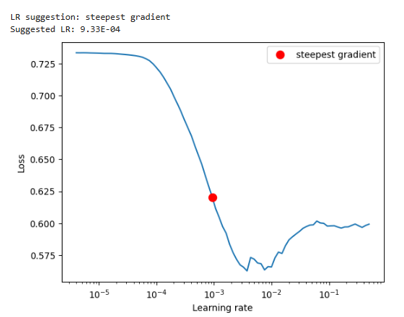
\includegraphics[width=0.58\textwidth]{figuras/LR_finder.png}
    \caption[Curva de busca de taxa de aprendizado]{Exemplo conceitual de curva usada em busca de taxa de aprendizado. A figura ilustra o tipo de análise; os valores finais devem ser extraídos dos relatórios atuais da Fase 7.}
    \label{fig:lr-finder}
\end{figure}

O otimizador padrão de triagem é AdamW \cite{loshchilov2019decoupled}. Precisão
mista está disponível, mas a configuração padrão atual é \texttt{fp32}; portanto
citações sobre AMP só devem ser usadas quando essa opção estiver habilitada
\cite{micikevicius2018mixed}. Quando ocorre divergência esperada, apenas o teste
ativo é encerrado e o histórico parcial é preservado para análise posterior.

\section{Treinamento supervisionado}\label{sec:met_treinamento}

A Fase 8 treina um modelo de segmentação por execução. As linhas de treino e
validação são resolvidas a partir do manifesto mestre, com opção de usar
\texttt{TRAIN\_SELECTED} apenas para treino. Antes da otimização, o estágio
confirma que os identificadores de paciente de treino e validação são disjuntos.

A perda combina BCE da classe positiva e termos Dice para fundo e primeiro
plano:
\begin{equation}
    \mathcal{L} =
    \alpha\,\mathcal{L}_{\mathrm{BCE},\mathrm{fg}}
    + \beta\,\mathcal{L}_{\mathrm{Dice},\mathrm{bg}}
    + \gamma\,\mathcal{L}_{\mathrm{Dice},\mathrm{fg}}.
    \label{eq:perda_treinamento}
\end{equation}
A família de perda é compatível com estratégias usadas em segmentação de WSI
\cite{khened2021generalized}; os pesos $\alpha$, $\beta$ e $\gamma$ são
parâmetros experimentais do repositório e devem ser reportados para cada
execução final.

Para avaliação durante treinamento, os logits são convertidos em probabilidades.
Em formulações multiclasse, a função softmax é:
\begin{equation}\label{eq:softmax}
    p_c = \mathrm{softmax}(\mathbf{z})_c =
    \frac{e^{z_c}}{\sum_{k=1}^{C}e^{z_k}},
\end{equation}
em que $\mathbf{z}$ é o vetor de logits e $C$ é o número de classes. Em seguida,
um limiar transforma probabilidades em máscara binária:
\begin{equation}\label{eq:binarizacao-threshold}
    \hat{g}_{j,i}(t)=
    \begin{cases}
        1, & \text{se } p_{j,i}\geq t,\\
        0, & \text{se } p_{j,i}<t.
    \end{cases}
\end{equation}

A seleção de checkpoints usa AUPRC de validação, métrica adequada a cenários
desbalanceados \cite{saito2015precision}. Métricas auxiliares incluem AUROC e
varredura de MCC \cite{fawcett2006roc,matthews1975comparison}. O treinamento
também rejeita épocas colapsadas, valores não finitos e validações sem amostras
válidas, reduzindo risco de preservar checkpoints cientificamente inválidos.

\section{Otimização do ensemble e inferência final}\label{sec:met_ensemble_inferencia}

A Fase 9 combina modelos individuais em uma receita de \textit{ensemble} usando
apenas pacientes de validação. A ideia geral é apoiada pela literatura de
\textit{ensemble learning} \cite{dietterich2000ensemble,caruana2004ensemble},
mas a implementação local usa pesos contínuos, limiares e busca por Optuna. A
receita produzida contém modelos, pesos, limiares, assinaturas de compatibilidade
e, quando configurado, TTA por espelhamento \cite{moshkov2020test}.

Se $M$ modelos produzem mapas de probabilidade $p_m(x)$, uma forma abstrata do
\textit{ensemble} ponderado é:
\begin{equation}\label{eq:ensemble}
    p_{\mathrm{ens}}(x)=
    \frac{\sum_{m=1}^{M} w_m p_m(x)}{\sum_{m=1}^{M} w_m},
\end{equation}
em que $w_m$ é o peso atribuído ao modelo $m$. A máscara final é obtida pela
comparação de $p_{\mathrm{ens}}(x)$ com um limiar calibrado na validação. Essa
calibração precisa ocorrer antes do teste.

A Fase 10 consome a receita congelada e avalia o conjunto de teste. Ela valida
assinaturas, carrega checkpoints, aplica a regra final de decisão e produz
métricas, figuras e relatórios. A fase não seleciona novos modelos nem reajusta
pesos ou limiares. Dice e IoU finais, quando reportados por contagens acumuladas,
seguem:
\begin{equation}
    \mathrm{Dice} = \frac{2TP}{2TP+FP+FN},
    \qquad
    \mathrm{IoU} = \frac{TP}{TP+FP+FN}.
    \label{eq:dice_iou}
\end{equation}
Quando houver pacientes suficientes, intervalos de confiança serão estimados por
reamostragem bootstrap de pacientes \cite{efron1979bootstrap}. Esses intervalos
descrevem variação empírica do conjunto avaliado e não substituem validação
externa.

\section{Limitações metodológicas conhecidas}\label{sec:met_limitacoes}

Quatro limitações permanecem explícitas até a versão final. Primeiro, os
identificadores de paciente usados para separação são os identificadores
operacionais persistidos no manifesto; sua equivalência biológica precisa ser
garantida pela origem dos dados. Segundo, VAHADANE \texttt{fixed\_source} é uma
aproximação por matriz fixa, não VAHADANE exato com ajuste por \textit{patch}.
Terceiro, a seleção GIST em grandes conjuntos deve ser descrita como
GIST-style. Quarto, resultados quantitativos só podem ser preenchidos a partir
dos artefatos consolidados das Fases 8 a 10.
